\begin{frame}[fragile]
    \frametitle{Example: Input Language for SageMath}
    {\centering\begin{adjustbox}{}
    \begin{lstlisting}
sage: g = AlternatingGroup(5)
sage: g.cardinality()
60
    \end{lstlisting}
    \end{adjustbox}\par
    \vspace{1em}
    \str{Let G be the alternating group on 5 symbols. What is the cardinality of G?}\par
}

    \vspace{2em}
    \begin{itemize}
        \item Can we make a natural input language for SageMath?\com{WolframAlpha-like}
        \item GLIF Prototype:
            \begin{itemize}
                \item Parsing
                \item Semantics construction translates to SageMath command (not logic)
            \end{itemize}
    \end{itemize}
\end{frame}

\begin{frame}
    \frametitle{Example: Input Language for SageMath -- Grammar}
    \centering
    \only<1>{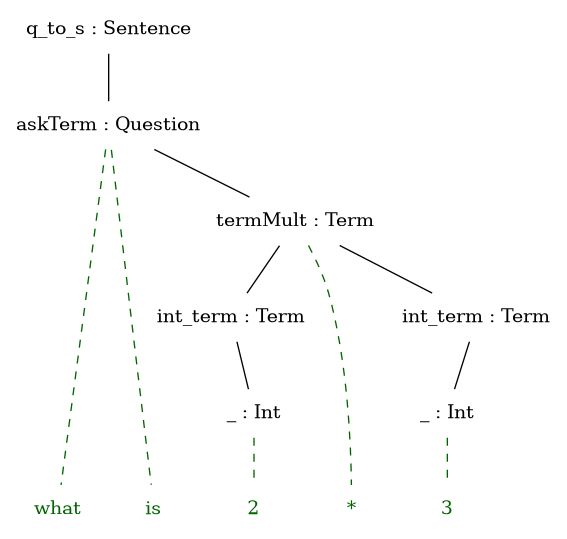
\includegraphics[scale=0.35]{img/glif-sage-ast-1.png}}
    \only<2>{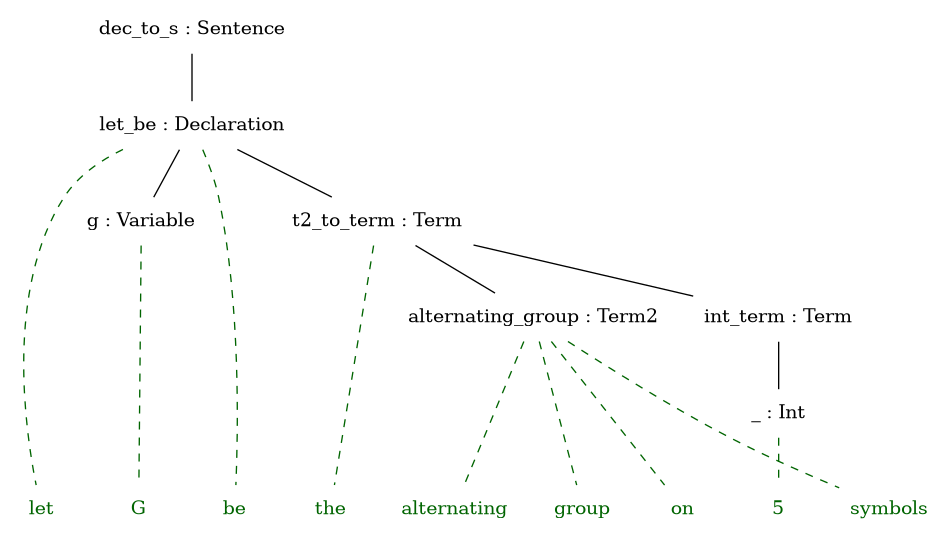
\includegraphics[scale=0.35]{img/glif-sage-ast-2.png}}
    \par
\end{frame}

\begin{frame}[fragile]
    \frametitle{Example: Input Language for SageMath -- Semantics Construction}
    \begin{itemize}
        \item Target logic: Python/SageMath commands
        \item Can experiment with ideas (e.g. notations)
    \end{itemize}

    \centering
    \onslide<1->{
        \vspace{1em}
        \str{let G be the alternating group on 5 symbols}\par
        $\downarrow$\par
        {\color{logicfg!50}assign gVar (alternating{\_}group (int{\_}term 5))}\par
        {\color{logicfg}\ttfamily g = AlternatingGroup(int(5))}\par
    }
    \onslide<2>{
        \vspace{2em}
        \str{let $|$ G $|$ be a notation for the cardinality of G}\par
        $\downarrow$\par
        {\color{logicfg}\ttfamily def bar(gVar): return gVar.cardinality()}\par
        \vspace{2em}
        \str{let D{\_}N be a notation for the dihedral group of order 2 * N}\par
    }
\end{frame}

\begin{frame}[fragile]
    \frametitle{Example: Input Language for SageMath}
    \lstset{basicstyle=\small\ttfamily,commentstyle={\sffamily\color{nlfg}},morecomment=[l]{Let},morecomment=[l]{What}}
    \begin{lstlisting}[columns=flexible]
Enter command: What are the Cayley tables of the alternating groups on 2 and 3 symbols?
    \end{lstlisting}
    \vskip-1em
    \begin{lstlisting}
print(AlternatingGroup(int(2)).cayley_table())
print(AlternatingGroup(int(3)).cayley_table())
sage:
*  a
 +--
a| a

sage:
*  a b c
 +------
a| a b c
b| b c a
c| c a b
    \end{lstlisting}
\end{frame}

\begin{frame}[fragile]
    \frametitle{Example: Input Language for SageMath}
    \begin{itemize}
        \item Took just a few hours to create prototype
        \item Maybe useful for teaching?
        \item GF made it easy to support another language (German)
        \item $\leadsto$ can also translate automatically:
    \end{itemize}

    \centering
    \vspace{1.5em}
    \str{What are the Cayley tables of the alternating groups on 2 and 3 symbols?}\par
    $\downarrow$\par
    \str{Was sind die Verkn\"upfungstafeln der alternierenden Gruppen \"uber 2 und 3 Elemente?}\par
\end{frame}

